\chapter{Sampling and Sampling Distributions}

\section{Population and Sample}

\begin{definition}[Population]
The totality of all possible outcomes or observations of a survey or experiment is called a population.
\end{definition}
A \textbf{sample} is a subset of a population. \\
Every outcome or observation can be recorded as a numerical or categorical value. Thus, each member of a population is a value of a random variable. There are two kinds of populations, namely, finite and infinite populations.
As the names suggest, a finite population consists of a finite number of elements (for example, the number of species of dogs) whereas an infinite population is one that consists of an infinitely (countable and uncountable) large number of elements (for example, the results of all possible rolls of a pair of dice).

\begin{note}
\end{note}
Some finite populations are so large that in theory we assume them to be infinite, such as the population lives of a certain type of storage battery being manufactured from a factory.

\section{Random Sampling}

\subsection{Simple Random Sampling}
A set of $n$ members taken from a given population is called a \textbf{sample} of size $n$.
\begin{definition}[Simple Random Sample]
A simple random sample of $n$ members is a sample that is chosen in such a way that every subset of $n$ observations of the population has the same probability of being selected. (Or, in other words, each sample point in the population has equal probability of being selected)
\end{definition}
If the process of selecting a sample is \textbf{random}, it is necessarily independent of other samples being drawn.
\subsection{Sampling without Replacement}
In general, there are $\dbinom{N}{n}$ samples of size $n$ that can be drawn from a finite population of size $N$ without replacement (we disregard the order of selection). Each sample has an equal chance of being selected. Hence, each sample has a probability of $\dfrac{1}{\binom{N}{n}}$ of being selected.
\subsection{Sampling with Replacement}
Here, the order of elements is taken into consideration (since 2 elements can appear in the outcome but be chosen in different orders). In general, there are $N^n$ samples of size $n$ that can be drawn from a finite population of size $N$ with replacement.Hence, each sample has a probability of $\dfrac{1}{N^n}$ of being selected
\subsection{Sampling from an Infinite Population (with/without replacement)}
We would be sampling from an infinite population if we sample with replacement from a finite population, and our sample would be random if
\begin{enumerate}
    \item in each draw, all the elements of the population have the same probability of being selected, and
    \item successive draws are independent.
\end{enumerate}
Even if we sample without replacement from an "infinite" population, removing one element from an infinite population does not affect the population. For example, if you have an equal number of infinite red and blue balls. If you draw a red ball in your first draw, the probability of drawing a red ball still remains equal to the blue ball (because you still have infinite red balls!).
\begin{note}
\end{note}
It is important to remember that within a population, there can be many repeated values and each is considered a separate data point. For example, consider the population of all NUS students. Say, we are interested in calculating their CAP. We know that the range of CAP is from 0 - 5 but we don't know the exact CAP of any student prior to sampling. Hence, this is a random variable. Further, multiple students may (in fact by Pigeonhole Principle, must) have the same CAP. We still consider them separate data points since they represent the CAP of different students. Just because the "values" are the same, it does not mean that the data points themselves are the same. 
\begin{note}
\end{note}
Selecting a sample without replacement from a finite population cannot be considered equivalent to sampling from an infinite population since the elements will get exhausted after a finite number of draws. In contrast, for an infinite population or
finite population with replacement, you are able to draw a sample as large as you want.
\begin{definition}[Random Sample]
Let $X$ be a random variable with certain probability distribution, $f_X(x)$. Let $X_1, X_2, \dots , X_n$ be $n$ independent random variables each having the same distribution as $X$, then $(X_1, X_2, \dots, X_n)$ is called a random sample of size $n$ from a population with distribution $f_X(x)$.\\
The joint p.f. (or p.d.f.) of $(X_1, X_2, \dots, X_n)$ is given by $f_{X_1, X_2, \dots, X_n}(x_1, x_2, \dots, x_n) = f_{X_1}(x_1)f_{X_2}(x_2) \dots f_{X_n}(x_n)$, where $f_X(x)$ is the p.f. (or p.d.f.) of the population.
\end{definition}

We say that $(X_1, X_2, \dots, X_n)$ is a random sample from a distribution with probability function $f_X(x)$. Here, a "random sample" is equivalent to  "$X_1, X_2, \dots, X_n$ are independent and identically distributed (i.i.d.)". So, a random sample of size $n$ can be represented by $n$ independent random variables that follow the same distribution. \\
Keep in mind that $X_{i}'s$ follow the same distribution (i.e., identically distributed) does not mean that $X_1 = X_2 = \dots = X_n$ (i.e., identical random variables). \\ You cannot say that $X + Y = 2X$ just because $X$ and $Y$ follow the same distribution. The actual realization of the random variables $X$ and $Y$ may be different even though they follow the same distribution!
Two random variables are equal if, and only if, they map \textbf{each} sample point to the same value. If Alice throws a die and Bob also throws a die, both the outcomes follow the same distribution. But, they are different random variables (if we are interested in the number showing up)! If Alice gets a 4, it does not mean that Bob also gets a 4.
\begin{note}[Motivation behind random sample, parameter, and statistic]
\end{note}
\begin{enumerate}
    \item The population parameter, say, $\mu$,  is \textbf{not observed}; but the values of $X_1, X_2, \dots, X_n$ are observed as $x_1, x_2, \dots, x_n$. So we hope to establish an "estimation rule" to estimate the unknown $\mu$ using the observed $X_1 = x_1, X_2 = x_2 \dots, X_n = x_n$; such a rule is called a statistic (say, $\bar{X} = \dfrac{1}{n}\sum_{i = 1}^n X_i$). In literature, $\bar{X}$ is also called an "estimator" for $\mu$. $\bar{x}$ is \textbf{computed/observed} based on the sample, and is called an estimate.
    \item Note that $\mu$ is an unknown constant - it is not a random variable. The population mean is fixed and constant - we just don't know the value because we haven't got data from the entire population.
    \item The statistic is a function of the sample; the fundamental requirement is that it does not depend on any unknown parameters. for example, $g_1(X_1, \dots, X_n) = 1$ is a statistic since it maps every input of samples to 1. But it is not a useful statistic.
    \item The statistical performance of the statistic decides which one is better to use in practice. In other words, we would be interested in studying the distribution of a statistic, called "sampling distribution". The sampling distribution is also crucial for the subsequent inference for the corresponding parameter.
    \item The sampling distribution for a statistic, say $\bar{X}$, is \textbf{not} how the sample $(X_1, X_2, \dots, X_n)$ performs. Instead, it is the distribution for the corresponding statistic (say, $\bar{X}$). So, constructing the histogram based on the observed $X_1 = x_1, X_2 = x_2, \dots, X_n = x_n$ to have a view of the sampling distribution of $\bar{X}$ is absolutely meaningless. Instead we should do the following:
    \begin{enumerate}
        \item Get the first sample $(X_1^{(1)}, X_2^{(1)}, \dots, X_n^{(1)})$ from the distribution $f_X(x)$, and compute the sample mean $\bar{X}^{(1)}$.
        \item Get the second sample $(X_1^{(3)}, X_2^{(2)}, \dots, X_n^{(2)})$ from the distribution $f_X(x)$, and compute the sample mean $\bar{X}^{(2)}$.
        \item Continue this procedure many times
        \item Get the $K^{th}$ sample $(X_1^{(K)}, X_2^{(K)}, \dots, X_n^{(K)})$ from the distribution $f_X(x)$, and compute the sample mean $\bar{X}^{(K)}$.
        \item Draw the histogram of $\bar{X}^{(1)}, \bar{X}^{(2)}, \dots, \bar{X}^{(n)}$
    \end{enumerate}
    \item In general, $\bar{X} \neq \mu$. $\bar{X}$ is a random variable and can have different realizations depending on the random sample drawn. But, $E[\bar{X}] = \mu$. It is important to understand this difference.
\end{enumerate}

\section{Sampling Distributions of Sample Mean}
Our main purpose in selecting random variables is to elicit information about the unknown population parameters.

\subsection{Statistic and Sampling Distribution}
A function of a random sample $(X_1, X_2, \dots, X_n)$ (which does not depend on any unknown quantities) is called a \textbf{statistic}. For example, $\bar{X}$ is a statistic as $\bar{X} = \dfrac{1}{n} \sum_{i = 1}^n X_i$. \\
Another example is $X_{median}$ or $X_{min}$. \\
But $V = \sum_{i = 1}^n \dfrac{(X_i - \mu)^2}{n - 1}$ is not a statistic if we do not know the population mean.\\
Hence, \textbf{a statistic is a random variable}. It is meaningful to consider the probability distribution of a statistic. The probability distribution of a statistic is called a \textbf{sampling distribution}.
\subsubsection{Sample Mean}
If $X_1, X_2, \dots, X_n$ represent a random sample of size $n$, then the sample mean is defined by the statistic
$$
\bar{X} = \dfrac{1}{n} \sum_{i = 1}^n X_i
$$
If the values in a random sample are observed and they are $x_1, x_2, \dots, x_n$, then the \textbf{realization} of the statistic $\bar{X}$ is given by 
$$\bar{x} = \dfrac{1}{n} \sum_{i = 1}^{n} x_i$$
We denote the population mean by $\mu_X$.

\thm{Sampling Distribution of the sample mean \\
For random samples of size $n$ taken from an infinite population or from a \textbf{finite population with replacement} having population mean $\mu$ and population standard deviation $\sigma$, the sampling distribution of the sample mean $\bar{X}$ has its mean and variance given by 
$$
\mu_{\bar{X}} = \mu_X \qquad \text{and} \qquad  \sigma_{\bar{X}}^2 = \dfrac{\sigma_{X}^2}{n}
$$, where $n$ is the sample size. In other words, 
$$
\mathbb{E}[\bar{X}] = \mathbb{E}[X] \qquad \text{and} \qquad  V(\bar{X}) = \dfrac{V(X)}{n}
$$}

\thm{Law of Large Numbers (LNN) \\
Let $X_1, X_2, \dots, X_n$ be a random sample of size $n$ from a population having any distribution with mean $\mu$ and finite population variance $\sigma^2$. Then for any $\epsilon \in \mathbb{R}$,
$$
P(|\bar{X} - \mu| > \epsilon) \xrightarrow{} 0 \text{ as } n \xrightarrow{} \infty
$$.}
This says that as the sample size increases, the probability that the sample mean differs from the population mean goes to zero. Another way of looking at this is that as $n$ gets larger, it is increasing likely that $\bar{X}$ is close to $\mu$. (The error between our estimated mean and the actual population mean gets smaller and smaller as we conduct sampling with larger and larger samples)
\begin{note}
\end{note}
The strong law of large numbers (also called Kolmogorov's law) states that the sample average converges almost surely to the expected value.
That is, $P(\lim_{n \xrightarrow{} \infty}\bar{X_n} = \mu ) = 1$
\begin{note}[Proof of LLN]
\end{note}
With Chebyshev's inequality, this theorem can be easily proved. Note that $\epsilon$ is an arbitrary but fixed constant. So, we have
$$
0 \leq P(|\bar{X} - \mu| > \epsilon) \leq \dfrac{V(\bar{X})}{\epsilon^2} = \dfrac{\sigma^2}{n \epsilon^2} \xrightarrow{} 0 \qquad \text{as } n \xrightarrow{} \infty
$$
The variance of the population should be finite for the expectation of the random variable $\bar{X}$ to converge to a fixed value. Obviously, $\mu$ must be finite since it is a fixed unknown constant. If variance were infinite,  $\bar{X}$ could assume infinitely many values (realizations) for different random samples and there is no guarantee that the expectation of all these values will be equal to the population mean.

\thm{Central Limit Theorem \\
Let $X_1, X_2, \dots, X_n$ be a random sample of size $n$ from. a population having any distribution with mean $\mu$ and finite population variance $\sigma^2$. The sampling distribution of the sample mean $\bar{X}$ is \textbf{approximately normal} with mean $\mu$ and variance $\dfrac{\sigma^2}{n}$ if $n$ is \textbf{sufficiently large}. Hence, 
$$
Z = \dfrac{\bar{X} - \mu}{\frac{\sigma}{\sqrt{n}}} \text{ follows approximately } N(0,1)
$$}
Note that the variance of the sampling distribution of the sample mean is at most equal to the population variance (since $n \geq 1$). \\
The above theorem is powerful in the sense that it tells us that the distribution of the sampling distribution will be normal if $n$ is large \textbf{no matter what the shape of the population distribution is}.
\begin{enumerate}
    \imp{ \item If for all $i = 1, 2, \dots, n$, $X_i$ are $N(\mu, \sigma^2)$, then $\bar{X}$ follows $N(\mu, \dfrac{\sigma^2}{n})$ regardless of the sample size $n$}
    \item Similarly, if \imp{for all $i = 1, 2, \dots, n$, $X_i$ are approximately $N(\mu, \sigma^2)$, then $\bar{X}$ approximately follows $N(\mu, \dfrac{\sigma^2}{n})$ regardless of the sample size $n$}
\end{enumerate}
Note that the above 2 points have nothing to do with the central limit theorem. With the normality assumption, the distribution of $\bar{X}$ is exactly normal. More generally, the linear combination of independent normal random variables with the same parameters is also a normal random variable (but obviously the parameters change).
If $X_1, X_2, \dots, X_n \sim N(\mu, \sigma^2)$, then $a_1 X_1 + a_2 X_2 + \dots + a_n X_n \sim N(\mu \sum_{i}^n a_i, \sigma^2 \sum_{i}^n a_i^2)$. Then, if you choose each of the $a_i$ to be equal to $\dfrac{1}{n}$, you get the first result.
\begin{note}
\end{note}
Central limit theorem only gives us the approximate distribution for $\bar{X}$, not the exact distribution. More rigorously, central limit theorem says that, for any $z \in \mathbb{R}$, 
$$
\lim_{n \xrightarrow{} \infty} P\left(\dfrac{\bar{X} - \mu)}{\sigma/\sqrt{n}} \leq z \right) = \Phi(z),
$$ where $\Phi(z)$ is the c.d.f. for the standard normal distribution.
So, practically, when $n$ is large, the distribution of $\dfrac{\bar{X} - \mu)}{\sigma/\sqrt{n}}$ is similar to that of a standard normal random variable. We normally use central limit theorem when $n \geq 30$ but this is not a fixed rule. If the actual distribution is quite symmetric, we can use it even for smaller values of $n$. The smaller the $n$, the less accurate the approximation.
\begin{note}
\end{note}
You must ensure that the distribution for which central limit theorem is being applied has a finite variance. For example, a Cauchy distribution has no mean or variance and so you cannot apply the central limit theorem.  Instead, any linear combination of Cauchy variables has a Cauchy distribution (so that the mean of a random sample of observations from a Cauchy distribution has a Cauchy distribution).
\begin{note}[Central Limit Theorem vs LLN]
\end{note}
Central Limit Theorem provides an approximate distribution of $\bar{X}$ (much more information). LLN provides a likely good estimate of $\mu$ based on $\bar{X}$ from a large sample but says nothing about the distribution.
\begin{note}
\end{note}
It is the distribution of $\bar{X}$ that follows approximately a normal distribution if $n$ is large. The underlying distribution of the population does not follow a normal distribution even if $n$ is large, i.e., $\bar{X}$ follows approximately normal as n is large but $X$ does not follow approximately normal even if the population size is very large. Each individual sample still follows the same underlying distribution that the population follows. For example, consider tossing a coin. Let the sample size be 1000. So, one sample consists of tossing a coin 1000 times and noting the number of heads and tails. Find the mean of the sample (assign 1 to head and 0 to tail). Now, repeat this procedure multiple times to get multiple sample means. When looking at the distribution of all the sample means, we expect it to follow a normal distribution but we don't expect each individual sample to follow a normal distribution. In particular, each sample is a Bernoulli distribution (with n = 1000 and p = 0.5). The sample mean is a normal distribution with mean = 0.5 (you are more likely to get 500 heads than 900 heads out of 1000 tosses).

\section{Sampling Distribution of the Difference of 2 Sample means}

\thm{\hfill \\
If independent samples of sizes $n_1$ ($\geq$ 30) and $n_2$ ($\geq$ 30) are drawn from two populations, with means $\mu_1$ and $\mu_2$, and variances $\sigma_1^2$ and $\sigma_2^2$ respectively, then the sampling distribution of the differences of the sample means, $\bar{X_1}$ and $\bar{X_2}$, is approximately normally distributed with mean and variance given by
$$
\mu_{\bar{X_1} - \bar{X_2}} = \mu_1 - \mu_2 \qquad \text{and} \qquad \sigma_{\bar{X_1} - \bar{X_2}}^2 = \dfrac{\sigma_1^2}{n_1} + \dfrac{\sigma_2^2}{n_2}
$$}
The proof the above theorem is relatively straightforward:
$$
\mu_{\bar{X_1} - \bar{X_2}} = E[\bar{X_1} - \bar{X_2}] = E[\bar{X_1}] - E[\bar{X_2}] = \mu_1 - \mu_2
$$
and 
$$
\sigma_{\bar{X_1} - \bar{X_2}}^2 = V(\bar{X_1} - \bar{X_2}) = V(\bar{X_1}) + V(\bar{X_2})
$$
since $\bar{X_1}$ and $\bar{X_2}$ are independent. Therefore, 
$$
\sigma_{\bar{X_1} - \bar{X_2}}^2 = \dfrac{\sigma_1^2}{n_1} + \dfrac{\sigma_2^2}{n_2}
$$
Since $\bar{X_1}$ and $\bar{X_2}$ are approximately normally distributed, therefore $\bar{X_1} - \bar{X_2}$ is also approximately normally distributed.
\begin{note}
\end{note}

\begin{enumerate}
    \item Note that if both $n_1, n_2 \geq 30$, the normal approximation for the distribution of $\bar{X_1} - \bar{X_2}$ is very good regardless of the shapes of the two population distributions.
    \item Recall that if a random variable $Y \sim N(\mu, \sigma^2)$, then $\dfrac{Y - \mu}{\sigma} \sim N(0,1)$. Similarly, here we have
    $$
    \dfrac{(\bar{X_1} - \bar{X_2}) - (\mu_1 - \mu_2)}{\sqrt{\dfrac{\sigma_1^2}{n_1} + \dfrac{\sigma_2^2}{n_2}}} \text{ approximately } \sim N(0,1) 
    $$
\end{enumerate}
We denote the sample standard deviation as $S$ and the sample variance as $S^2$. Further, we denote the population standard deviation as $\sigma$ and population variance as $\sigma^2$.

\section{Chi-Square Distribution}

\begin{definition}[Chi-Square Distribution]
If $Y$ is a random variable  with p.d.f.
$$
f_Y(y) = \begin{cases}
\dfrac{1}{2^{n/2}\Gamma(n/2)} y^{n/2 - 1} e^{-y/2} \text{, for } y > 0 \\
0 \text{, otherwise}
\end{cases}
$$ then $Y$ is said to have a chi-squared distribution with $n$ degrees of freedom, denoted by $\chi^2(n)$, where $n$ is a positive integer, and $\Gamma(.)$ is the gamma function. \\
\end{definition}
The gamma function, $\Gamma(.)$ is defined by 
$$
\Gamma(n) = \int_{0}^{\infty} x^{n-1} e^{-x} dx = (n-1)!
$$ for $n = 1, 2, 3, \dots $
\begin{figure}
    \centering
    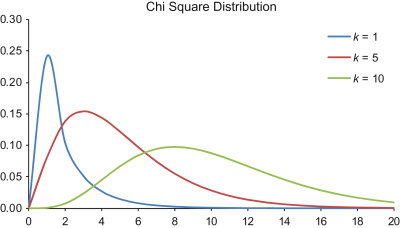
\includegraphics{Images/Chi-squared distribution.jpg}
    \caption{Chi-squared distribution}
    \label{fig:my_label}
\end{figure}
\begin{note}[Some Properties of Chi-square distributions]
\end{note}
\begin{enumerate}
    \item If $Y \sim \chi^2(n)$, then $E[Y] = n$ and $V(Y) = 2n$.
    \item For large $n$, $\chi^2(n)$ approx $\sim N(n,2n)$.
    \item If $Y_1, Y_2, \dots, Y_k$ are \textbf{independent} chi-squared random variables with $n_1, n_2, \dots, n_k$ degrees of freedom respectively, then $Y_1 + Y_2 + \dots + Y_K$ has chi-square distribution with $n_1 + n_2 + \dots + n_k$ degrees of freedom. That is, $\sum_{i = 1}^k Y_i \sim \chi^2 \left( \sum_{i = 1}^k n_i\right)$
\end{enumerate}

\thm{\hfill \\
\begin{enumerate}
    \item If $X \sim N(0,1)$, then $X^2 \sim \chi^2(1)$
    \item Let $X \sim N(\mu, \sigma^2)$, then $[(X - \mu)/\sigma]^2 \sim \chi^2(1)$
    \item Let $X_1, X_2, \dots, X_n$ be a random sample from a normal population with mean $\mu$, and variance $\sigma^2$. Define
    $$
    Y = \sum_{i = 1}^n \dfrac{(X_i - \mu)^2}{\sigma^2}
    $$
    Then $Y \sim \chi^2(n)$
\end{enumerate}}
Let $c$ be a constant satisfying $P(Y \geq c) = \int_{c}^{\infty} f_Y(y) dy = \alpha$, where $Y \sim \chi^2(n)$. We use the notation $\chi^2(n; \alpha)$ to denote this constant $c$. That is, $P(Y \geq \chi^2(n; \alpha)) = \int_{\chi^2(n; \alpha)}^{\infty} f_Y(y) dy = \alpha$. \\
Similarly, $\chi^2(n; 1 - \alpha)$ is the constant satisfying $P(Y \leq \chi^2(n; 1 - \alpha)) = \int_{0}^{\chi^2(n; 1 - \alpha)} f_Y(y)dy = \alpha$

\section{The Sampling Distribution of $(n-1)S^2/\sigma^2$}
Let $X_1, X_2, \dots, X_n$ be a random sample from a population. Then the statistic
$$
S^2 = \dfrac{1}{n - 1} \sum_{i = 1}^n (X_i - \bar{X})^2
$$ is called the sample variance.
The sampling distribution of the random variable $S^2$ has little practical application in statistics. \\
Instead, we shall consider the sampling distribution of the random variable $\dfrac{(n-1)S^2}{\sigma^2}$ when $X_i \sim N(\mu, \sigma^2)$ for all $i$.

\thm{\hfill \\
If $S^2$, is the variance of a random sample of size $n$ taken from a \textbf{normal} population having the variance $\sigma^2$, then the random variable $\dfrac{(n-1)S^2}{\sigma^2}$ has a \textbf{chi-squared distribution with $n - 1$ degrees of freedom.} That is, $\dfrac{(n-1)S^2}{\sigma^2} \sim \chi^2(n-1)$}

\section{The t-distribution}
\begin{figure}
    \centering
    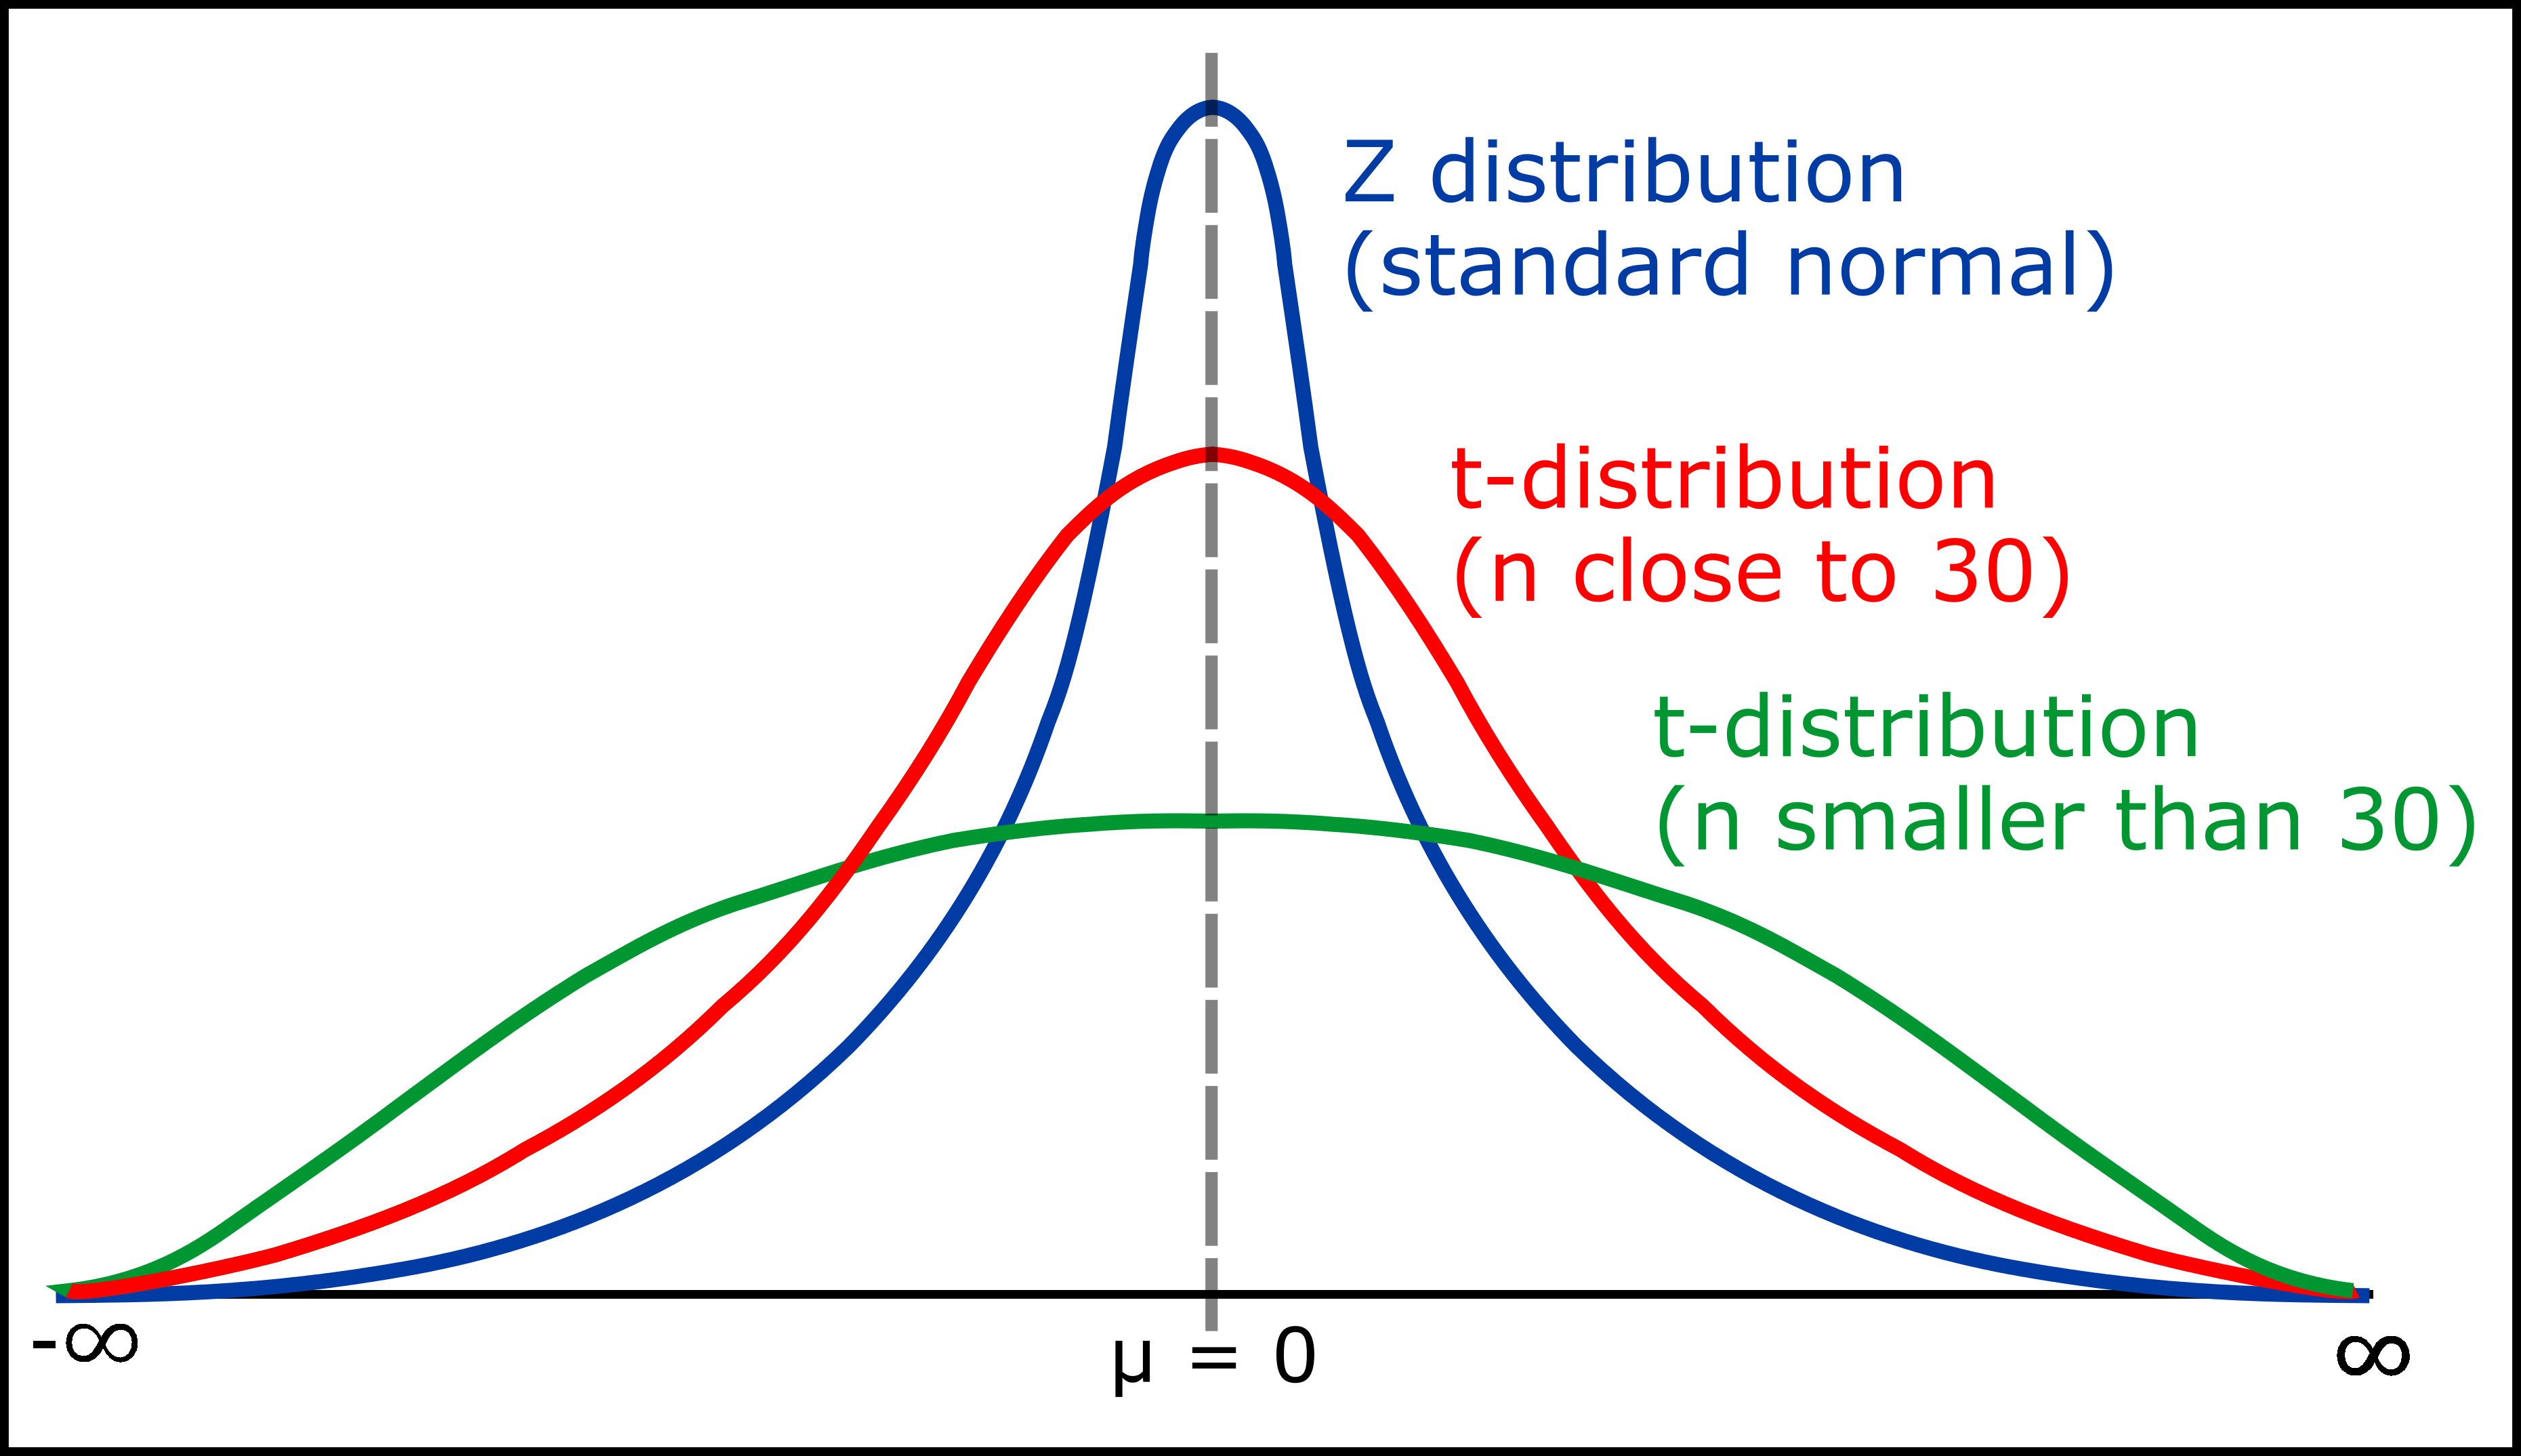
\includegraphics[width = 10cm]{Images/t-distribution.png}
    \caption{t-distribution}
    \label{fig:my_label}
\end{figure}
\begin{definition}[t-distribution]
Suppose $Z \sim N(0,1)$ and $U \sim \chi^2(n)$. If $Z$ and $U$ are \textbf{independent}, and let $T = \dfrac{Z}{\sqrt{U/n}}$ then the random variable $T$ follows the t-distribution with $n$ degrees of freedom. That is, $\dfrac{Z}{\sqrt{U/n}} \sim t(n)$
\end{definition}
If $T$ follows a t-distribution with $n$ degrees of freedom, then its p.d.f. is given by 
$$
f_T(t) = \dfrac{\Gamma \left( \dfrac{n + 1}{2}\right)}{\sqrt{n\pi}\Gamma(n/2)} \left( 1 + \dfrac{t^2}{n}\right)^{\dfrac{n+1}{2}}, \qquad -\infty < t < \infty
$$
where the gamma function is defined as earlier.

\begin{note}
\end{note}
\begin{enumerate}
    \item The graph of the t-distribution is symmetric about the vertical axis and resembles the graph of the standard normal distribution.
    \item It can be shown that the p.d.f. of t-distribution with $n$ d.f. (degrees of freedom) is approaching to the p.d.f. of standard normal distribution when $n \xrightarrow{} \infty$. That is, 
    $$
    \lim_{n \xrightarrow{} \infty} f_T(t) = \dfrac{1}{\sqrt{2\pi}} e^{-t^2 / 2}
    $$ as $n \xrightarrow{} \infty$
    \item The values of $P(T \geq t) = \int_{t}^{\infty} f_T(x) dx$ for selected values of $n$ and $t$ are given in a statistical table.
    \item If $T \sim t(n),$ then $E[T] = 0$ and $V(T) = \dfrac{n}{n - 2}$ for $n > 2$.
\end{enumerate}

\begin{note}
\end{note}
If the random sample was selected from a normal population, then
$$
Z = \dfrac{(\bar{X} - \mu)}{\sigma/\sqrt{n}} \sim N(0,1)
$$ and
$$
U = \dfrac{(n-1)S^2}{\sigma^2} \sim \chi^2(n-1)
$$
It can be shown that $\bar{X}$ and $S^2$ are independent, and so are $Z$ and $U$.
Therefore, 
\begin{equation*}
    \begin{split}
        T &= \dfrac{\bar{X} - \mu }{S/\sqrt{n}} \\
        &= \dfrac{(\bar{X} - \mu)/(\sigma/\sqrt{n})}{\sqrt{\dfrac{(n-1)S^2}{\sigma^2}/(n-1)}} \sim t_{n-1}
    \end{split}
\end{equation*}
That is, $T$ has a t-distribution with $n - 1$ d.f. (degrees of freedom).
Observe the relation between $Z, U, T$ closely. If you replace the $\sigma$ (Population standard deviation) in $Z$ with $S$ (Sample standard deviation), the distribution changes from standard normal to t-distribution with $n - 1$ degrees of freedom.
\section{The F-distribution}
\begin{figure}
    \centering
    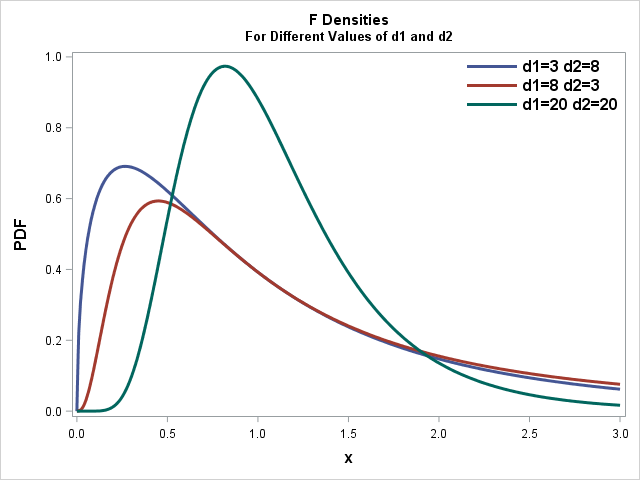
\includegraphics[width = 10cm]{Images/F-distribution.png}
    \caption{F-distribution}
    \label{fig:my_label}
\end{figure}

\begin{definition}[The F-distribution]
Let $U$ and $V$ be independent random variables having $\chi^2(n_1)$ and $\chi^2(n_2)$ respectively. Then, the distribution of the random variable $F = \dfrac{U/n_1}{V/n_2}$, is called a $F$-distribution with $(n_1, n_2)$ degrees of freedom. \\
Observe that $F$ is the ratio of 2 $\chi^2$ random variables, each adjusted by its respective degrees of freedom. Moreover, the parameters of the F-distribution are precisely the degrees of freedom of the 2 $\chi^2$ random variables (first of the random variable in the numerator, then that of the one in the denominator) \\
The p.d.f of $F$ is given by 
$$
f_F(x) = 
\begin{cases}
\dfrac{n_1^{n_1/2}n_2^{n_2/2}\Gamma(\dfrac{n_1 + n_2}{2})}{\Gamma(\dfrac{n_1}{2})\Gamma(\dfrac{n_2}{2})} \dfrac{x^{n_1 / 2 - 1}}{(n_1 x + n_2)^{(n_1 + n_2)/2}}, \text{ for } x > 0 \\
0, \text{ otherwise}
\end{cases}
$$
\end{definition}
It can be shown that 
\begin{equation*}
    \begin{split}
        E[X] &= \dfrac{n_2}{n_2 - 2}, \text{ with } n_2 > 2 \\
        V(X) &= \dfrac{2n_2^2 (n_1 + n_2 - 2)}{n_1(n_2 - 2)^2(n_2 - 4)}, \text{ with } n_2 > 4
    \end{split}
\end{equation*}

\thm{\hfill \\
If $F \sim F(n,m)$, then $\dfrac{1}{F} \sim F(m,n)$}
This theorem follows immediately from the definition of F-distribution. Recall that $F = \dfrac{U/n_1}{V/n_2}$. Then, $\dfrac{1}{F} = \dfrac{V/n_2}{U/n_1}$ follows $F(n_2, n_1)$. \\
Values of the F-distribution can be found in the statistical tables. The table gives the values of $F(n_1, n_2; \alpha)$ such that $P(F > F(n_1, n_2; \alpha)) = \alpha$. For example, $F(5,4; 0.05) = 6.26$ means that $P(F > 6.26) = 0.05$, where $F \sim F(5,4)$.

\thm{
$$
F(n_1, n_2; 1 - \alpha) = \dfrac{1}{F(n_2, n_1; \alpha)}
$$}
Here is a short proof: Let $F \sim F(n_1, n_2)$, then $\dfrac{1}{F} \sim F(n_2, n_1)$, Based on the definition of $F(n_1, n_2; 1 - \alpha)$,
$$
P(F > F(n_1, n_2; 1 - \alpha)) = 1 - \alpha,
$$ which leads to 
$$
P(F < F(n_1, n_2; 1 - \alpha)) = 1 - P(F > F(n_1, n_2; 1 - \alpha)) = \alpha
$$
That is,
$$
P\left(\dfrac{1}{F} > \dfrac{1}{F(n_1, n_2; 1 - \alpha)} \right) = \alpha,
$$
which together with the fact that $\dfrac{1}{F} \sim F(n_2, n_1)$ implies
$$
\dfrac{1}{F(n_1, n_2; 1 - \alpha)} = F(n_2, n_1, \alpha)
$$
\begin{note}
\end{note}
Checking the definition of $t$ and $F$ distributions, we find one important connection between them: If $Y \sim t(n)$, then $Y^2 \sim F(1,n)$
\section{Summary of Sampling Distributions}
\begin{enumerate}
    \item If $X_1, X_2, \dots, X_n$ are $N(\mu, \sigma^2)$, then $\dfrac{\bar{X} - \mu}{\sigma/\sqrt{n}}$ follows $N(0,1)$ regardless of the sample size $n$. If $X_1, X_2, \dots, X_n$ have mean $\mu$ and finite variance $\sigma^2$ and $n$ is sufficiently large, then $\dfrac{\bar{X} - \mu}{\sigma/\sqrt{n}}$ approximately follows the $N(0,1)$ standard normal distribution.
    \item If $X_1, X_2, \dots, X_n$ are $N(\mu, \sigma^2)$, then $\dfrac{(n -1)S^2}{\sigma^2} \sim \chi^2(n-1)$, where $S^2$ is the sample variance of the random sample.
    \item If $X_1, X_2, \dots , X_n$ are $N(\mu, \sigma^2)$, then $\dfrac{\bar{X} - \mu }{S/\sqrt{n}} \sim t(n-1)$.
    \item Let $X_{1,1}, X_{1,2}, \dots, X_{1,n_1}$ be $N(\mu_1, \sigma_1^2)$ and let $X_{2,1}, X_{2,2} \dots, X_{2,n_2}$ be $N(\mu_2, \sigma_2^2)$. Denote by $S_1^2$ and $S_2^2$ the sample variances of $X_{1,1}, X_{1,2}, \dots, X_{1,n_1}$ and $X_{2,1}, X_{2,2} \dots, X_{2,n_2}$ respectively. Then, we have $\dfrac{S_1^2/\sigma_1^2}{S_2^2/\sigma_2^2} \sim F(n_1 - 1 , n_2 - 1)$.
\end{enumerate}